\subsection{Blurring an Image}
\label{sect:blur}

In this task, you will write a function to blur an image. The core of this
transformation is this function:
\begin{quote}
\begin{lstlisting}
pixel_t[] blur(pixel_t[] pixels, int width, int height,
               int[] mask, int maskwidth)
\end{lstlisting}
\end{quote}
The returned array should be the representation of the blurred image.

\paragraph{Masks}
In addition to an input image, we pass the blur transformation a
\emph{mask}, an $n \times n$ array of non-negative integers
representing \emph{weights}.  For our purposes, $n$ must be odd. This
means that the $n \times n$ array has a well defined center --- the
\emph{origin}.  While weights in the mask can be 0 (but not negative),
the weight in the center position of the mask cannot be zero.

For each pixel in the input image, think of the mask as being placed
on top of the image so its origin is on the pixel we wish to
alter. The original intensity value of each pixel under the mask is
multiplied by the corresponding value in the mask that covers it.
These products are added together, and then we divide by the total of
the weights in the mask to get the intensity of the output pixel. Always
use the original (input) values for each pixel for each mask calculation, not
the output values you compute as you create the new image.


\begin{figure}
  \begin{minipage}[c]{0.6\textwidth}\centering
    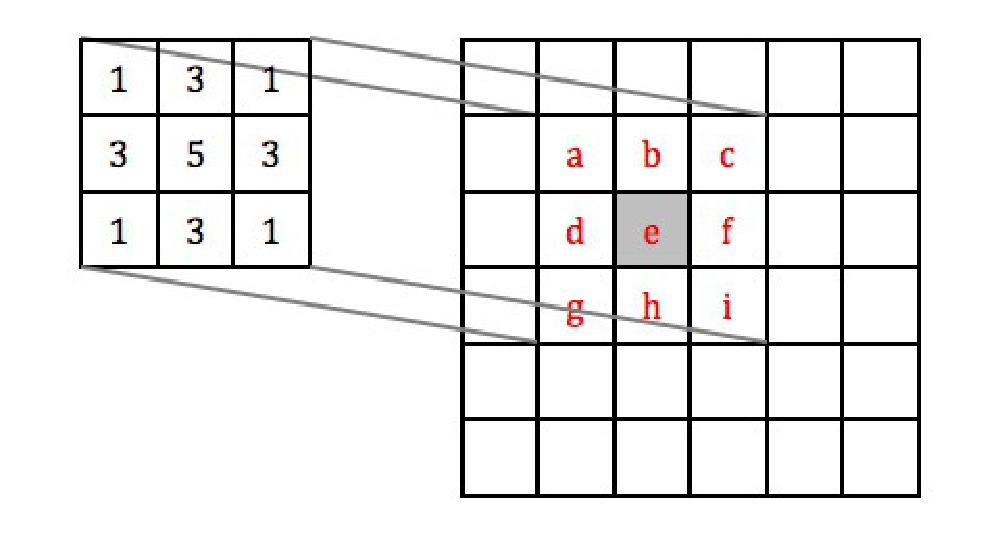
\includegraphics[scale=0.45]{\img/blurexample-eps-converted-to.pdf}
  \end{minipage}\hfill
  \begin{minipage}[c]{0.37\textwidth}
    \caption{Overlay the $3 \times 3$ mask over the image so it is centered on
      pixel $e$ to compute the new value for pixel $e$.}
    \label{fig:blur-exampleA}
  \end{minipage}
\end{figure}

\begin{figure}
  \begin{minipage}[c]{0.6\textwidth}\centering
    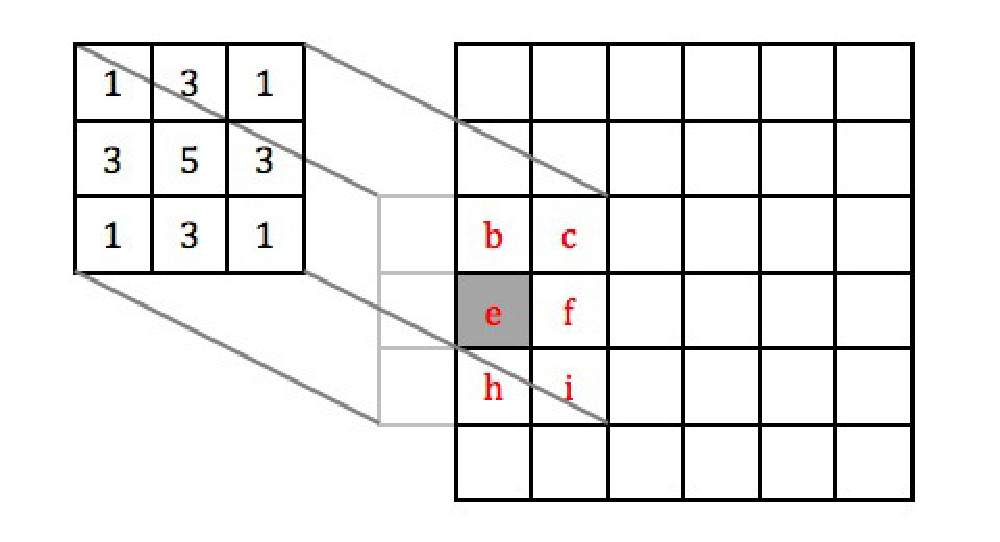
\includegraphics[scale=0.45]{\img/blurexample2-eps-converted-to.pdf}
%% The integer in index 18 of the returned array should be
%% \lstinline'3b + c + 5e + 3f + 3h + i'\\ where \lstinline'b' is the average intensity
%% of the pixel labeled \lstinline'b' and so on.
  \end{minipage}\hfill
  \begin{minipage}[c]{0.37\textwidth}
    \caption{If the mask hangs over the edge of the image, use only those mask
      values that cover the image in the weighted sum.}
    \label{fig:blur-exampleB}
  \end{minipage}
\end{figure}
% \begin{figure}[t]
%   \begin{minipage}[c]{0.67\textwidth}\centering
%     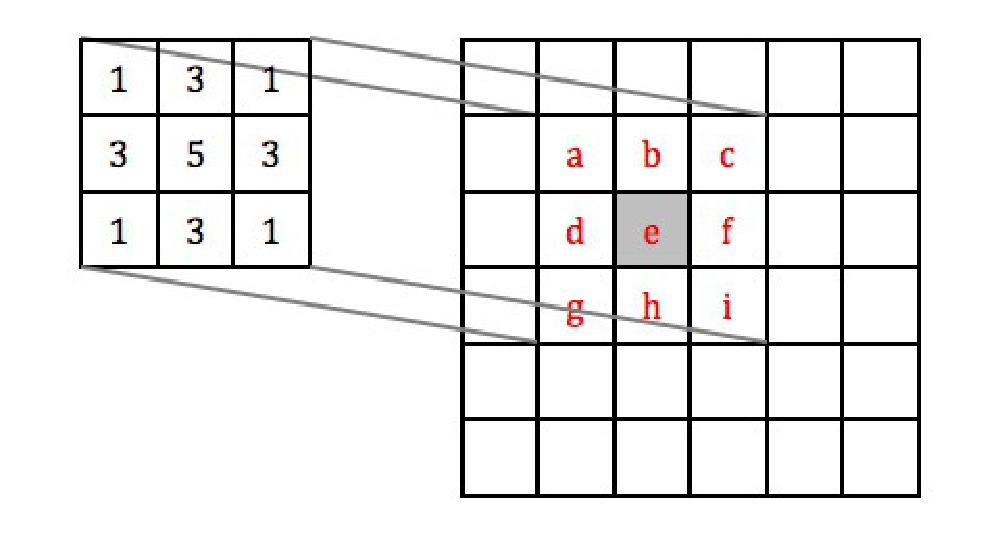
\includegraphics[scale=0.45]{\img/blurexample-eps-converted-to.pdf}
%   \end{minipage}\hfill
%   \begin{minipage}[c]{0.3\textwidth}
%     \caption{Overlay the $3 \times 3$ mask over the image so it is centered on
%       pixel $e$ to compute the output value corresponding to pixel $e$.}
%     \label{fig:blur-example}
%   \end{minipage}
% \end{figure}

For example, refer to Figure~\ref{fig:blur-exampleA}, which shows a $3 \times
3$ mask and an image that we want to blur. Suppose we want to compute the
output intensity value based on pixel \lstinline'e'.  Imagine overlaying the
mask so its center position is on \lstinline'e'.  We would compute the output
intensity for \lstinline'e' as:

\begin{quote}
\begin{lstlisting}
(a + 3b + c + 3d + 5e + 3f + g + 3h + i)  / 21
\end{lstlisting}
\end{quote}
This calculation is done three times for each pixel, once for its red channel,
once for its green channel, and once for its blue channel. Do not apply the
transformation to the alpha channel of the pixel.

% \begin{figure}
%   \begin{minipage}[c]{0.67\textwidth}\centering
%     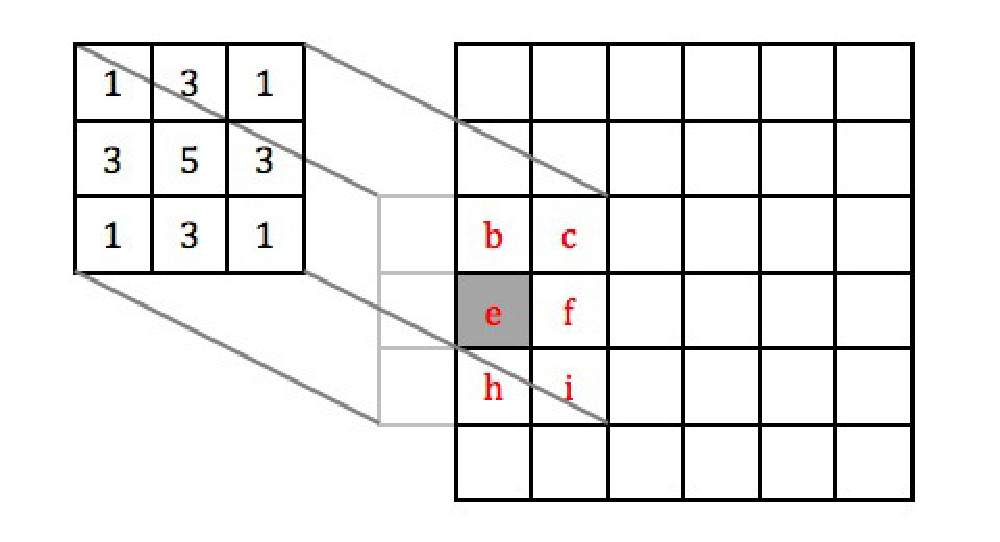
\includegraphics[scale=0.45]{\img/blurexample2-eps-converted-to.pdf}
%   \end{minipage}\hfill
%   \begin{minipage}[c]{0.3\textwidth}
%     \caption{If the mask hangs over the edge of the image, use only those mask
%       values that cover the image in the weighted sum.}
%     \label{fig:blur-example2}
%   \end{minipage}
% \end{figure}


Note that sometimes when you center the mask over a pixel you want to
blur, the mask will hang over the edge of the image. In this case,
compute the weighted sum of only those pixels the mask covers. In
these cases, you must divide by the sum of only those weights that you
use from the mask. For the example shown in
Figure~\ref{fig:blur-exampleB}, the output intensity for the pixel
\lstinline'e' is given by:
\begin{quote}
\begin{lstlisting}
(3b + c + 5e + 3f + 3h + i)  / 16
\end{lstlisting}
\end{quote}

\begin{figure}[b]
\centering

\includegraphics[scale=1]{\img/scs.png}
\quad

\includegraphics[scale=1]{\img/scs-blur-slightly.png}
\quad

\includegraphics[scale=1]{\img/scs-blur.png}
\caption{The SCS Dragon: original image (left), blurred slightly with
  a $3 \times 3$ mask (middle), and blurred with a $5 \times 5$ mask
  (right). See text for mask values.}
\label{fig:carnegie-blur}
\end{figure}


Figure~\ref{fig:carnegie-blur} shows a sample image blurred using the
following masks, which are given in the handout as
\lstinline'blur-slightly-mask.txt' and \lstinline'blur-mask.txt',
respectively:
\begin{verbatim}
         1 3 1          1 2 3 2 1
         3 5 3          2 3 4 3 2
         1 3 1          3 4 5 4 3
                        2 3 4 3 2
                        1 2 3 2 1
\end{verbatim}

The \lstinline'mask' passed to the function must have width $n \times
n$, where $n$ is given by the argument \lstinline'maskwidth'.  If the
supplied image does not match the size given by \lstinline'width' and
\lstinline'height', or if the mask is not a square matching the size
given by \lstinline'maskwidth', or if \lstinline'maskwidth' is not
odd, or if the mask contains negative integers or a zero at the
origin, your program should abort with a precondition failure when
compiled and run with the \lstinline'-d' flag.

\begin{task}[10]
\TAGS{array, safety, testing}
Create a C0 file \lstinline'blur.c0' implementing a function
\lstinline'blur'. You may include any auxiliary functions you need in the
same file, but you should not include a \lstinline'main()' function.
\end{task}

You should look at \lstinline'README.txt' to see how to compile and run
this transformation against \lstinline'blur-main.c0'. You are also strongly
encouraged to write some test cases for your programs in a
file \lstinline'images-test.c0'.



%%% Local Variables:
%%% mode: latex
%%% TeX-master: "main"
%%% End:
